%% (Master) Thesis template
% Template version used: v1.4
%
% Largely adapted from Adrian Nievergelt's template for the ADPS
% (lecture notes) project.


%% We use the memoir class because it offers a many easy to use features.
\documentclass[11pt,a4paper,titlepage]{memoir}

%% Packages
%% ========

%% LaTeX Font encoding -- DO NOT CHANGE
\usepackage[OT1]{fontenc}

%% Babel provides support for languages.  'english' uses British
%% English hyphenation and text snippets like "Figure" and
%% "Theorem". Use the option 'ngerman' if your document is in German.
%% Use 'american' for American English.  Note that if you change this,
%% the next LaTeX run may show spurious errors.  Simply run it again.
%% If they persist, remove the .aux file and try again.
\usepackage[english]{babel}

%% Input encoding 'utf8'. In some cases you might need 'utf8x' for
%% extra symbols. Not all editors, especially on Windows, are UTF-8
%% capable, so you may want to use 'latin1' instead.
\usepackage[utf8]{inputenc}

%% This changes default fonts for both text and math mode to use Herman Zapfs
%% excellent Palatino font.  Do not change this.
\usepackage[sc]{mathpazo}

%% The AMS-LaTeX extensions for mathematical typesetting.  Do not
%% remove.
\usepackage{amsmath,amssymb,amsfonts,mathrsfs}

%% NTheorem is a reimplementation of the AMS Theorem package. This
%% will allow us to typeset theorems like examples, proofs and
%% similar.  Do not remove.
%% NOTE: Must be loaded AFTER amsmath, or the \qed placement will
%% break
\usepackage[amsmath,thmmarks]{ntheorem}

%% LaTeX' own graphics handling
\usepackage{graphicx}

%% We unfortunately need this for the Rules chapter.  Remove it
%% afterwards; or at least NEVER use its underlining features.
\usepackage{soul}

%% This allows you to add .pdf files. It is used to add the
%% declaration of originality.
\usepackage{pdfpages}

%% Some more packages that you may want to use.  Have a look at the
%% file, and consult the package docs for each.
%% See the TeXed file for more explanations

%% [OPT] Multi-rowed cells in tabulars
%\usepackage{multirow}

%% [REC] Intelligent cross reference package. This allows for nice
%% combined references that include the reference and a hint to where
%% to look for it.
\usepackage{varioref}

%% [REC] Allow graphics files with spaces in their names
\usepackage{grffile}

%% [OPT] Easily changeable quotes with \enquote{Text}
%\usepackage[german=swiss]{csquotes}

%% [REC] Format dates and time depending on locale
\usepackage{datetime}

%% [OPT] Provides a \cancel{} command to stroke through mathematics.
%\usepackage{cancel}

%% [NEED] This allows for additional typesetting tools in mathmode.
%% See its excellent documentation.
\usepackage{mathtools}

%% [ADV] Conditional commands
%\usepackage{ifthen}

%% [OPT] Manual large braces or other delimiters.
%\usepackage{bigdelim, bigstrut}

%% [REC] Alternate vector arrows. Use the command \vv{} to get scaled
%% vector arrows.
\usepackage[h]{esvect}

%% [NEED] Some extensions to tabulars and array environments.
\usepackage{array}

%% [OPT] Postscript support via pstricks graphics package. Very
%% diverse applications.
%\usepackage{pstricks,pst-all}

%% [?] This seems to allow us to define some additional counters.
%\usepackage{etex}

%% [ADV] XY-Pic to typeset some matrix-style graphics
%\usepackage[all]{xy}

%% [OPT] This is needed to generate an index at the end of the
%% document.
%\usepackage{makeidx}

%% [OPT] Fancy package for source code listings.  The template text
%% needs it for some LaTeX snippets; remove/adapt the \lstset when you
%% remove the template content.
\usepackage{listings}
\lstset{language=TeX,basicstyle={\normalfont\ttfamily}}

%% [REC] Fancy character protrusion.  Must be loaded after all fonts.
\usepackage[activate]{pdfcprot}

%% [REC] Nicer tables.  Read the excellent documentation.
\usepackage{booktabs}


%% Our layout configuration.  DO NOT CHANGE.
%% Memoir layout setup

%% NOTE: You are strongly advised not to change any of them unless you
%% know what you are doing.  These settings strongly interact in the
%% final look of the document.

% Dependencies
\usepackage{ETHlogo}

% Turn extra space before chapter headings off.
\setlength{\beforechapskip}{0pt}

\nonzeroparskip
\parindent=0pt
\defaultlists

% Chapter style redefinition
\makeatletter

\if@twoside
  \pagestyle{Ruled}
  \copypagestyle{chapter}{Ruled}
\else
  \pagestyle{ruled}
  \copypagestyle{chapter}{ruled}
\fi
\makeoddhead{chapter}{}{}{}
\makeevenhead{chapter}{}{}{}
\makeheadrule{chapter}{\textwidth}{0pt}
\copypagestyle{abstract}{empty}

\makechapterstyle{bianchimod}{%
  \chapterstyle{default}
  \renewcommand*{\chapnamefont}{\normalfont\Large\sffamily}
  \renewcommand*{\chapnumfont}{\normalfont\Large\sffamily}
  \renewcommand*{\printchaptername}{%
    \chapnamefont\centering\@chapapp}
  \renewcommand*{\printchapternum}{\chapnumfont {\thechapter}}
  \renewcommand*{\chaptitlefont}{\normalfont\huge\sffamily}
  \renewcommand*{\printchaptertitle}[1]{%
    \hrule\vskip\onelineskip \centering \chaptitlefont\textbf{\vphantom{gyM}##1}\par}
  \renewcommand*{\afterchaptertitle}{\vskip\onelineskip \hrule\vskip
    \afterchapskip}
  \renewcommand*{\printchapternonum}{%
    \vphantom{\chapnumfont {9}}\afterchapternum}}

% Use the newly defined style
\chapterstyle{bianchimod}

\setsecheadstyle{\Large\bfseries\sffamily}
\setsubsecheadstyle{\large\bfseries\sffamily}
\setsubsubsecheadstyle{\bfseries\sffamily}
\setparaheadstyle{\normalsize\bfseries\sffamily}
\setsubparaheadstyle{\normalsize\itshape\sffamily}
\setsubparaindent{0pt}

% Set captions to a more separated style for clearness
\captionnamefont{\sffamily\bfseries\footnotesize}
\captiontitlefont{\sffamily\footnotesize}
\setlength{\intextsep}{16pt}
\setlength{\belowcaptionskip}{1pt}

% Set section and TOC numbering depth to subsection
\setsecnumdepth{subsection}
\settocdepth{subsection}

%% Titlepage adjustments
\pretitle{\vspace{0pt plus 0.7fill}\begin{center}\HUGE\sffamily\bfseries}
\posttitle{\end{center}\par}
\preauthor{\par\begin{center}\let\and\\\Large\sffamily}
\postauthor{\end{center}}
\predate{\par\begin{center}\Large\sffamily}
\postdate{\end{center}}

\def\@advisors{}
\newcommand{\advisors}[1]{\def\@advisors{#1}}
\def\@department{}
\newcommand{\department}[1]{\def\@department{#1}}
\def\@thesistype{}
\newcommand{\thesistype}[1]{\def\@thesistype{#1}}

\renewcommand{\maketitlehooka}{\noindent\ETHlogo[2in]}

\renewcommand{\maketitlehookb}{\vspace{1in}%
  \par\begin{center}\Large\sffamily\@thesistype\end{center}}

\renewcommand{\maketitlehookd}{\vfill\par}

\checkandfixthelayout

\setlength{\droptitle}{-48pt}

\makeatother

% This defines how theorems should look. Best leave as is.
\theoremstyle{plain}
\setlength\theorempostskipamount{0pt}

%%% Local Variables:
%%% mode: latex
%%% TeX-master: "thesis"
%%% End:


%% Theorem environments.  You will have to adapt this for a German
%% thesis.
%% Theorem-like environments

%% This can be changed according to language. You can comment out the ones you
%% don't need.

\numberwithin{equation}{chapter}

%% German theorems
%\newtheorem{satz}{Satz}[chapter]
%\newtheorem{beispiel}[satz]{Beispiel}
%\newtheorem{bemerkung}[satz]{Bemerkung}
%\newtheorem{korrolar}[satz]{Korrolar}
%\newtheorem{definition}[satz]{Definition}
%\newtheorem{lemma}[satz]{Lemma}
%\newtheorem{proposition}[satz]{Proposition}

%% English variants
\newtheorem{theorem}{Theorem}[chapter]
\newtheorem{example}[theorem]{Example}
\newtheorem{remark}[theorem]{Remark}
\newtheorem{corollary}[theorem]{Corollary}
\newtheorem{definition}[theorem]{Definition}
\newtheorem{lemma}[theorem]{Lemma}
\newtheorem{proposition}[theorem]{Proposition}

%% Proof environment with a small square as a "qed" symbol
\theoremstyle{nonumberplain}
\theorembodyfont{\normalfont}
\theoremsymbol{\ensuremath{\square}}
\newtheorem{proof}{Proof}
%\newtheorem{beweis}{Beweis}


%% Helpful macros.
%% Custom commands
%% ===============

%% Special characters for number sets, e.g. real or complex numbers.
\newcommand{\C}{\mathbb{C}}
\newcommand{\K}{\mathbb{K}}
\newcommand{\N}{\mathbb{N}}
\newcommand{\Q}{\mathbb{Q}}
\newcommand{\R}{\mathbb{R}}
\newcommand{\Z}{\mathbb{Z}}
\newcommand{\X}{\mathbb{X}}

%% Fixed/scaling delimiter examples (see mathtools documentation)
\DeclarePairedDelimiter\abs{\lvert}{\rvert}
\DeclarePairedDelimiter\norm{\lVert}{\rVert}

%% Use the alternative epsilon per default and define the old one as \oldepsilon
\let\oldepsilon\epsilon
\renewcommand{\epsilon}{\ensuremath\varepsilon}

%% Also set the alternate phi as default.
\let\oldphi\phi
\renewcommand{\phi}{\ensuremath{\varphi}}


%% Make document internal hyperlinks wherever possible. (TOC, references)
%% This MUST be loaded after varioref, which is loaded in 'extrapackages'
%% above.  We just load it last to be safe.
\usepackage[linkcolor=black,colorlinks=true,citecolor=black,filecolor=black]{hyperref}


%% Document information
%% ====================

\title{Project B. Permutation-invariant variational network for 2D+time cardiac image reconstruction}
\author{Oscar Kläsi}
\thesistype{Bonus Project}
\advisors{Advisors: Prof.\ Dr.\ A. D. Visor, Dr.\ P. Ostdoc}
\department{Department of Computer Science}
\date{June 11, 2025}

\begin{document}

\frontmatter

%% Title page is autogenerated from document information above.  DO
%% NOT CHANGE.
\begin{titlingpage}
  \calccentering{\unitlength}
  \begin{adjustwidth*}{\unitlength-24pt}{-\unitlength-24pt}
    \maketitle
  \end{adjustwidth*}
\end{titlingpage}


%% TOC with the proper setup, do not change.
\cleartorecto
\tableofcontents
\mainmatter

%% Your real content!
% Additional macros
\newcommand{\package}{\emph}

\chapter{Introduction}

The goal of Project B is to develop a permutation-invariant Variational Network (VN) for 2D + time cardiac image reconstruction. In real applications time frames can be out of order.

\section{Description}

I tried out different variational networks with different numbers of layers to see how much detail a deeper network can catch. To account for the permutation-invariant timeframes a vectorial total variation (VTV) regulariser is used to exploit the similarity of the timeframes of each batch. The Fourier transform in the VN leaves the time dimension untouched and the VTV is the only way the time domain is taken into account.

The program is designed so that every necessary parameter can easily be changed in a ``Hyperparameter'' section, including the regulariser and the loss function.

\subsection{Training}

The training was conducted on an 80/20 training validation split with two possible loss types.

\paragraph{Data Fidelity Loss}

The standard data fidelity loss proposed in the project script with \verb|USE_DEEP_SUPERVISION = False|:
\[
\min_{\Theta} \; \mathbb{E}_{(x,s,M)\sim\mathcal{T}}\;\bigl\lVert x_{\Theta}^{K}(s,M) - x \bigr\rVert_{1}
\]

\paragraph{Deep Supervision Loss}

The data fidelity loss embedded in a deep supervision manner\footnote{See lecture notes 9.} with \verb|USE_DEEP_SUPERVISION = True|:
\[
\mathcal{L}_{\text{total}} = \sum_{k=1}^K \exp(-\tau (K - k)) \cdot \left\| \mathbf{x}^{(k)} - \mathbf{x}_{\text{GT}} \right\|_1
\]

\subsection{Regularisers}

Three regularisers are available.

\paragraph{VTV}
The VTV regulariser proposed in the project script
\[
\text{Reg}^k(\mathbf{x}^k)_t = \sum_{i \le n_f} \mathbf{D}^{k,i^T} \left\{ (\mathbf{D}^{k,i}\mathbf{x}_t) \odot \varphi^{k,i} \left( \sqrt{\frac{|\mathbf{D}^{k,i}\mathbf{x}_1|^2 + \cdots + |\mathbf{D}^{k,i}\mathbf{x}_T|^2}{T}} \right) \right\}
\]

\paragraph{TV}
The isotropic TV regulariser introduced in lecture 5
\[
\|\nabla x\|_1 = \sum_p \sqrt{(\nabla_1x)^2 + (\nabla_2x)^2}
\]

\paragraph{Tikhonov}
\[
\text{tikhonov}(\mathbf{x}) = \mathbf{x} * \mathbf{K}, \qquad \mathbf{K} = \begin{bmatrix} 0 & -1 & 0 \\ -1 & 4 & -1 \\ 0 & -1 & 0 \end{bmatrix}
\]

\subsection{Choose Parameters}

I tried 3, 5 and 10 layers for the following fixed parameters.

\begin{description}
  \item[Network Parameters] \verb|N_LAYERS = 3,5,10|, \verb|N_FILTERS = 5|, \verb|FILTER_SZ = 3|, \verb|REGULARISER = "vtv"|
  \item[Undersampling and noise] \verb|NOISE_STD = 0.05|, \verb|ACCEL_RATE = 4|, \verb|CENTER_FRACTION = 0.1|, \verb|SIGMA = 10|
  \item[Training] \verb|BATCH_SIZE = 4|, \verb|NUM_EPOCHS = 15|, \verb|LR = 1e-2|, \verb|PRINT_EVERY = 10|, \verb|TRAIN_SPLIT = 0.8|, \verb|DS_TAU = 0.1|, \verb|USE_DEEP_SUPERVISION = True|, \verb|SHOW_VAL_IMAGES = True|
\end{description}

\begin{figure}[h]
  \centering
  \includegraphics[width=0.45\linewidth]{data/training_loss_different_n_layers.png}
  \caption{Training and validation loss for fixed parameters with different number of layers.}
\end{figure}

\begin{figure}[h]
  \centering
  \includegraphics[width=0.45\linewidth]{data/nRMSE_loss.png}
  \caption{nRMSE for fixed parameters with different number of layers.}
\end{figure}

The loss decreased for deeper networks as expected. Increasing the number of filters further decreases the loss. However, increasing the kernel size caused the network to converge slower; the epochs had to be increased from 15 to 25 to see convergence and the loss was still higher than for the other combinations. Due to limited computation capacity most experiments used a lower number of layers and filters.

\begin{figure}[h]
  \centering
  \includegraphics[width=0.45\linewidth]{data/training_validation_differnt_n_filter.png}
  \caption{Training and validation loss for different numbers of filters and kernel sizes.}
\end{figure}

\begin{figure}[h]
  \centering
  \includegraphics[width=0.45\linewidth]{data/mRMSE_different_n_filrters_size.png}
  \caption{nRMSE for different numbers of filters and kernel sizes.}
\end{figure}

\begin{figure}[h]
  \centering
  \includegraphics[width=0.45\linewidth]{data/learning_loss 1.png}
  \caption{Training loss for a 4\,x\,4 kernel with 10 layers, 5 filters and 25 epochs.}
\end{figure}

\begin{figure}[h]
  \centering
  \includegraphics[width=0.45\linewidth]{data/reconstruction loss.png}
  \caption{Training loss for a 3\,x\,3 kernel with 10 layers, 5 filters and 25 epochs.}
\end{figure}

\chapter{Experimental Setting}

The experimental setting consists only of the dataset \verb|2dt_heart.mat| that contains 2D + time ground truth images with shape $(128, 128, 11, 375)$. The first two dimensions are spatial, the third is the time dimension and the fourth corresponds to the samples. Synthetic data is created by adding an under-sampling mask and noise. From this training pairs a training and validation split with 80\% training and 20\% validation data is generated.

\section{Mask Generation}

Masks are generated randomly for each sample and provided to the VN. A fixed center radius is used and outside of this kernel a Laplace shaped density distribution with tuneable parameters is applied:
\[
  p(k_y) = \alpha \exp \left( -\frac{|k_y - n_y/2|}{\sigma} \right)
\]

\chapter{Results}

\section{VTV vs\ TV regulariser}

Comparing the VTV regulariser with Total Variation (TV) and Tikhonov regularisers shows notable differences. Training is much faster for TV and Tikhonov since they only look at one timeframe at a time, whereas VTV checks all frames. TV converges at about two epochs and Tikhonov after one epoch, while VTV starts to converge only after about 13 epochs with the same hyperparameters.

Hyperparameters were identical except for the regulariser.

\begin{description}
  \item[Network Parameters] \verb|N_LAYERS = 8|, \verb|N_FILTERS = 5|, \verb|FILTER_SZ = 3|, \verb|REGULARISER = "vtv" or "tv"|
  \item[Undersampling and noise] \verb|NOISE_STD = 0.05|, \verb|ACCEL_RATE = 4|, \verb|CENTER_FRACTION = 0.1|, \verb|SIGMA = 10|
  \item[Training] \verb|BATCH_SIZE = 4|, \verb|NUM_EPOCHS = 15|, \verb|LR = 1e-2|, \verb|PRINT_EVERY = 10|, \verb|TRAIN_SPLIT = 0.8|, \verb|DS_TAU = 0.1|, \verb|USE_DEEP_SUPERVISION = True|, \verb|SHOW_VAL_IMAGES = True|
\end{description}

\begin{figure}[h]
  \centering
  \includegraphics[width=0.45\linewidth]{data/2 - Zettelkasten/1 - Atomic Notes/Assets/learning_loss.png}
  \caption{VTV training $\ell_1$ loss.}
\end{figure}

\begin{figure}[h]
  \centering
  \includegraphics[width=0.45\linewidth]{data/training_loss 3.png}
  \caption{Tikhonov training $\ell_1$ loss.}
\end{figure}

\begin{figure}[h]
  \centering
  \includegraphics[width=0.45\linewidth]{data/tv_training_loss.png}
  \caption{TV training loss.}
\end{figure}

The VN with the VTV regulariser achieved a training loss of 0.019454, a validation loss of 0.019311 and an nRMSE of 0.092765. The Tikhonov version had a training loss of 0.029170, a validation loss of 0.029245 and an nRMSE of 0.140566. The TV version had higher losses as well (values not recorded).

\begin{figure}[h]
  \centering
  \includegraphics[width=0.45\linewidth]{data/training_loss_vtv_vs_tv.png.png}
  \caption{Training loss for VTV and TV regularisers for different noise and acceleration parameters.}
\end{figure}

\begin{figure}[h]
  \centering
  \includegraphics[width=0.45\linewidth]{data/validation_loss_vtv_vs_tv.png}
  \caption{Validation error (nRMSE) for VTV and TV regularisers for different noise and acceleration parameters.}
\end{figure}

\section{Deep Supervision vs no deep supervision}

The VN with deep supervision reached a training loss of 0.019391, validation loss of 0.019653 and an nRMSE of 0.094850. The VN without deep supervision achieved a training loss of 0.018163, a validation loss of 0.018055 and an nRMSE of 0.084516. The deep supervision model converged faster but the final performance was worse.

Hyperparameters:
\begin{description}
  \item[Network Parameters] \verb|N_LAYERS = 8|, \verb|N_FILTERS = 5|, \verb|FILTER_SZ = 3|, \verb|REGULARISER = "vtv"|
  \item[Undersampling and noise] \verb|NOISE_STD = 0.05|, \verb|ACCEL_RATE = 4|, \verb|CENTER_FRACTION = 0.1|, \verb|SIGMA = 10|
  \item[Training] \verb|BATCH_SIZE = 4|, \verb|NUM_EPOCHS = 25|, \verb|LR = 1e-2|, \verb|PRINT_EVERY = 10|, \verb|TRAIN_SPLIT = 0.8|, \verb|DS_TAU = 0.1|, \verb|USE_DEEP_SUPERVISION = True/False|, \verb|SHOW_VAL_IMAGES = True|
\end{description}

\begin{figure}[h]
  \centering
  \includegraphics[width=0.45\linewidth]{data/training_loss 8.png}
  \caption{Training loss of the VN with deep supervision.}
\end{figure}

\begin{figure}[h]
  \centering
  \includegraphics[width=0.45\linewidth]{data/training_loss 9.png}
  \caption{Training loss of the VN without deep supervision.}
\end{figure}

\begin{figure}[h]
  \centering
  \includegraphics[width=0.45\linewidth]{data/reconstruction_example 10.png}
  \caption{Example reconstruction images (without deep supervision).}
\end{figure}

\begin{figure}[h]
  \centering
  \includegraphics[width=0.45\linewidth]{data/reconstruction_example 9.png}
  \caption{Example reconstruction images (without deep supervision).}
\end{figure}

\chapter{Discussion}

The VTV regulariser that renders the 2D VN permutation invariant performs much better than regularisers that do not take the time dimension into account. Surprisingly, the VN with deep supervision performed worse than the VN without.

The parameters were chosen to keep the limited computation power and a reasonable runtime in mind. Future experiments could explore deeper networks and whether deep supervision still performs worse for more complex architectures.

\chapter{Bibliography}

All information used in this project are available in the course ``Model- and Learning-Based Inverse Problems in Imaging''. Generative AI was used for coding assistance.



\backmatter

\bibliographystyle{plain}
\bibliography{refs}

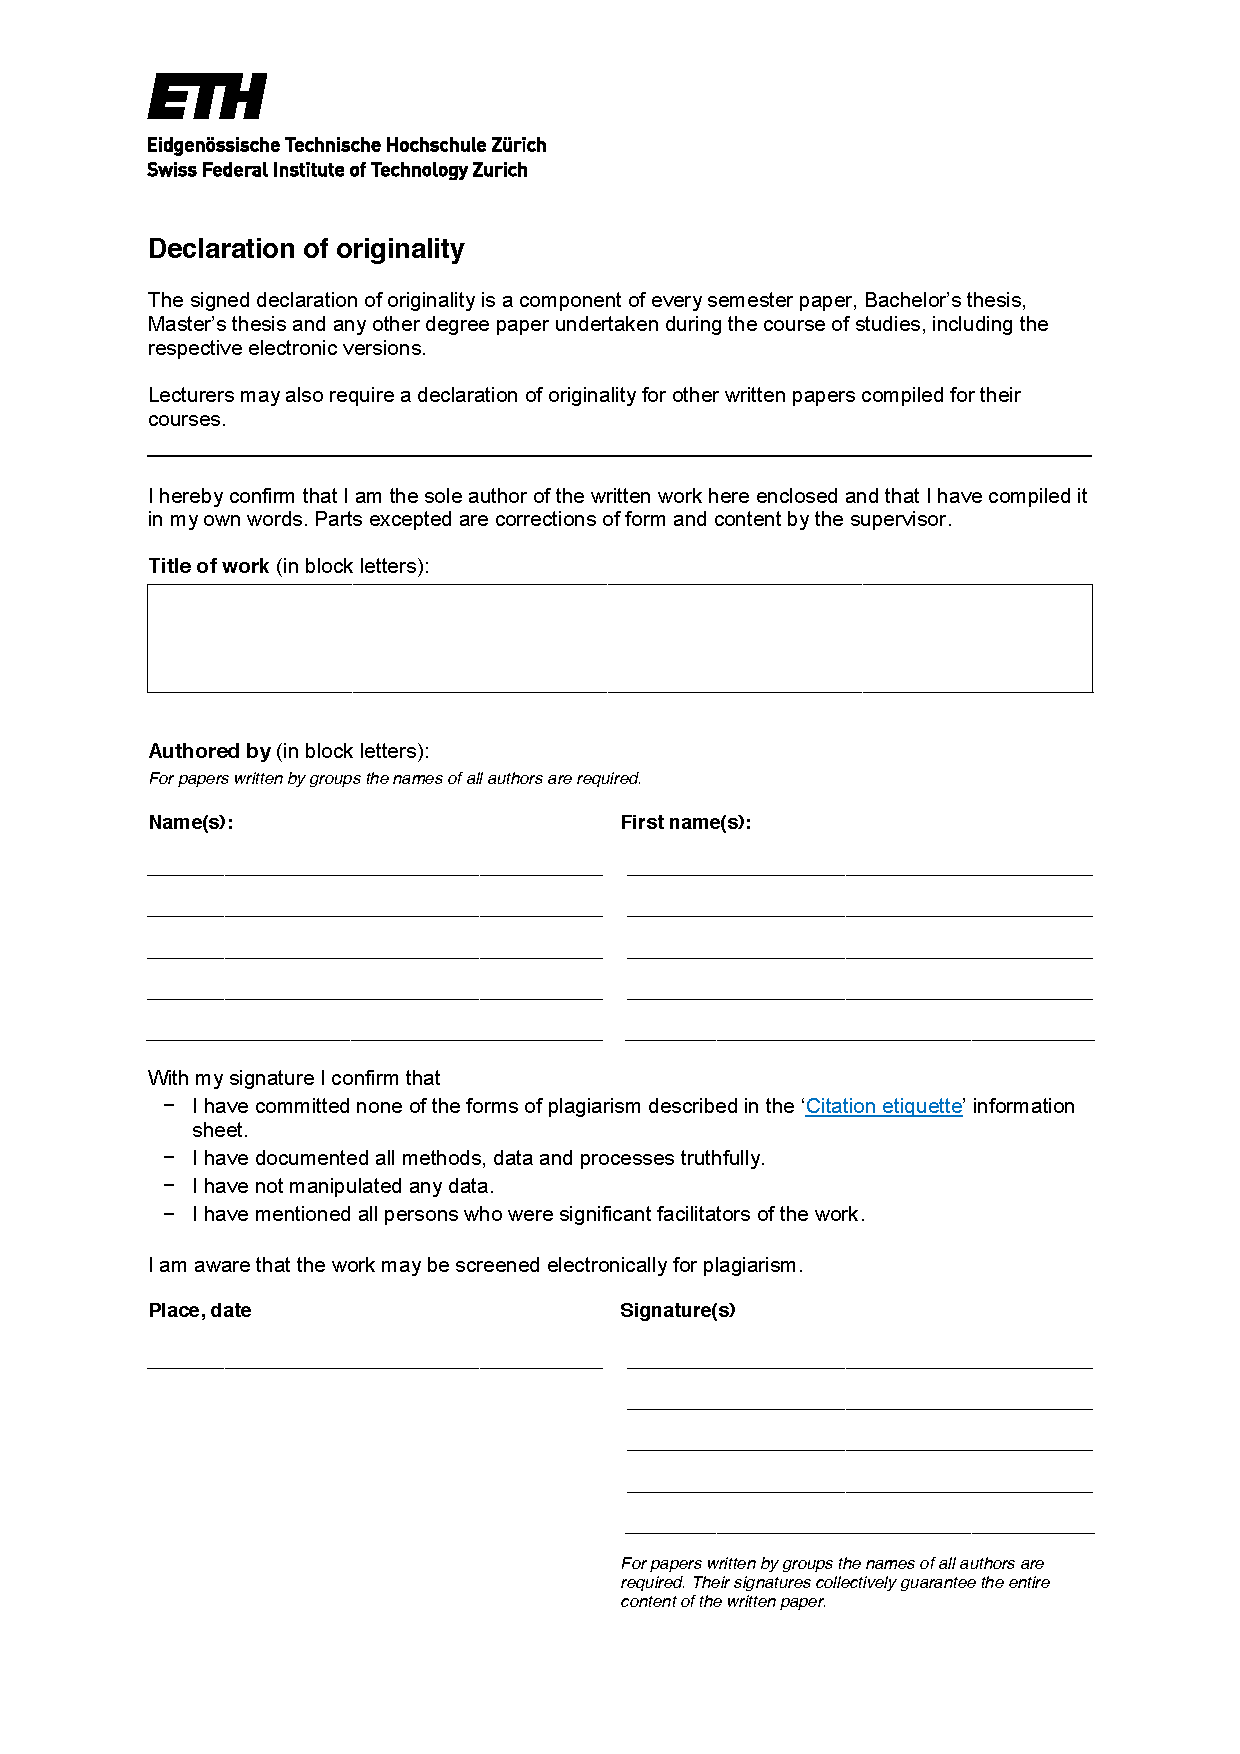
\includepdf[pages={-}]{declaration-originality.pdf}

\end{document}
